\begin{savequote}
Behaviour is the mirror in which everyone shows their image.
\qauthor{Johann Wolfgang von Goethe}
\end{savequote}


\chapter[Multiple Culture NVC Regression]{Multiple Culture NVC Regression}
\label{ChapterNvcRegression}

\thesiscomment{MAIN POINT: Cultural differences make training and testing on different cultures problematic, and we solve this by having culture specific automatic systems to improve performance.}

\thesiscomment{WHAT we do}

\thesiscomment{HOW we do it}

\thesiscomment{RESULTS, IMPACT and NOVELTY}

The previous chapter has described the collection of \ac{NVC} signal annotations from three cultures: Great Britain (GBR), Kenya (KEN) and India (IND). This chapter will now apply this data to automatic \ac{NVC} regression. The three cultures present in the annotation data are treated as three separate ground truth sets. The annotation data is not combined into a global label set because this results in a label set that does not reflect the annotator perceptions (see Table \ref{MeanAnnotatorCorrelationTable}). This is because \culturallySpecific annotation data better reflects the annotator perception of \ac{NVC} used to create the data set (see Section \ref{SectionAnalysisOfCultureAnnotation}). Also, discrete groups of annotators enables us to train an \ac{NVC} recognition system with one culture's annotation set and test it using a different culture. This will experimentally show the performance of using training data that is dissimilar to the test culture. Most emotion and \ac{NVC} studies do not consider cultural differences but it is expected that the training and test data needs to culturally correspond to achieve good performance. This raises a potential problem, if current methods are deployed in different cultures without appropriately accounting for cultural difference. 
%This chapter demonstrates a possible solution to this issue: to train classifiers on a specific culture to better model that culture's specific properties. This will result in better performance in a wider range of potential applications.

The work builds upon the \ac{NVC} classifier described in Chapter \ref{ChapterClassification}, but changes are introduced to address some of the previous chapter's shortcomings. In summary, these improvements are:

\begin{itemize}
 \item use of \continuous labels, which makes this task a regression problem,
 \item use all the samples in the corpus, including intermediate intensity \ac{NVC} and examples of disagreement, rather than just the clear samples,
 \item use of a slightly different machine learning technique: $\nu$-SVR (pronounced nu-SVR),
 \item use of annotation data from three distinct cultures,
 \item the performance is evaluated by Pearson's correlation,
 \item only a single feature set is used (\textit{geometric-a}), 
 \item clips of various lengths are summarised into a fixed length ``digest'' vector by taking the feature mean and variance and
 \item only person independent testing is performed.
\end{itemize}

%These changes, their justifications and their implications will now be discussed.

In Chapter \ref{ChapterClassification}, the problem was simplified to two classes by considering only clear examples of each \ac{NVC} signal. This greatly reduces the amount of available training data. Every sample in the corpus is used in this chapter, with \continuous labels (see Section \ref{SectionSelectionOfNvcCategories}). This increases the difficulty of the task because intermediate strength \ac{NVC}s can be difficult to distinguish. This has previously been discussed, with respect to gaze and \textit{thinking}, in Section \ref{SectionVisualisingGaze}.

Because \ac{NVC} recognition is now expressed as a regression problem, different machine learning techniques must be used. Adaboost and standard \ac{SVM}s are binary classifiers and cannot be directly applied. Other techniques may be applied to regression, such as $\nu$-SVR \cite{Scholkopf2000} and this is described in the next section.

Three \culturallySpecific annotation sets are used, spanning four \ac{NVC} signals (\textit{agree}, \textit{thinking}, \textit{question} and \textit{understand}).
%Following from the definition of $\filteredAnnotation$ in the previous chapter, each video clip has a label matrix $\filteredAnnotation_{\cultureSelect} \in \mathbb{R}^{3 \times 4}$. 
%This significantly differs from most other supervised learning problems in that they are usually considered as a single value or class label. 
%This label matrix may be regressed by considering each component separately and training a regressor on each. For a label matrix of size $3$ by $4$, 
For the 3 cultures and 4 \ac{NVC} categories, $3\cdot4=12$ separate regression models are constructed and evaluated independently. It would be desirable achieve a good overall performance because an effective method should generalise to many different types of \ac{NVC} and operate in different cultures.

Feature tracking and feature extraction are used to transform digital frames into a form usable for effective machine learning. The method used is based on computing a statistical features based on the mean and variance of individual feature components. This encodes general activity level and facial expression without encoding the order of events. A statistical feature is a feature that is based on the statistical properties of a set of unordered observations. Statistical features are also known as temporal features \cite{Chantler1997, Meng2007, Mognon2010}, as well as ensemble features.
Only a single \featureGeneration approach is used in this chapter (\textit{geometric-a}), to limit the number of experiments to a manageable scale. This technique was selected because it had the highest overall performance and generalised well to unseen subjects in Chapter \ref{ChapterClassification}. 
%Polynomial \temporalFeatSingle were not used because they only provide a marginal improvement in classification performance (see Section \ref{SectionTemporalFeatures}). 
%Instead of using frame and clip level comparisons to measure a system's performance, a frame features from each clip are combined to form a clip digest vector of fixed length.

The approach involves \ac{NVC} regression of each label component based on a distinct, culture and \ac{NVC} specific models. There may be a wide range of possible interpretations for perceiving and interpreting \ac{NVC} (see Section \ref{BackgroundWhatFactorsInfluenceNvc}) because interpretation is dependent on context. 
%It is important to remember there is no ``wrong way'' to perceive \ac{NVC}. 
Given the number of potential factors that can affect perception, the number of specialised models may become too large to create or use in a practical application.
%To achieve a realistic model of human \ac{NVC} perception, it may be necessary to have person specific \ac{NVC} perception models. Given the vast resources required to construct billions of models, it is reasonable to ask if this approach is reasonable. A similar issue might be raise for automatic emotion recognition, if everyone expresses happiness in a slightly different fashion depending on many possible influences. 
However, the problem is not as insurmountable as it may at first appear. 
\begin{itemize}
 \item For a specific application of automatic \ac{NVC} recognition, there are probably a limited range of social and cultural situations which will be of interest.
 \item There are culturally and socially based similarities between humans, which greatly reduces the scale of the task.
 \item General models can be used as a basis and adapted to users during a brief, person specific training session. A similar approach is used in automatic speech recognition, in which a general model is adapted to a user's unique style of speaking.
\end{itemize}

Although it would be a vast undertaking to comprehensively solve the problem in every situation, \ac{NVC} recognition based on specific groups of annotators and in a specific application is feasible.

The main contributions of this chapter are:
\begin{itemize}
\item A study of recognition based on culturally distinct sets of annotators to better model \culturallySpecific \ac{NVC} perception. The automatic system uses \continuous \ac{NVC} labels which provide richer information content than discrete labels.
\item An analysis of the effect of training with one culture's annotations and testing on a different culture's annotation data.
\end{itemize}

The next section discusses the existing studies relevant to this work. Section \ref{SectionRegressionSystemOverview} provides an overview of the automatic system. Section \ref{SectionDigestVector} discusses how \temporalFeatSingle{ }are extracted and how regression is applied. Results are presented and discussed in Section \ref{SectionRegressionResultsAndDiscussion}.

\section{Related Research}
\label{BackgroundSupervisedRegression}

This section reviews the literature relating to facial analysis regression, temporal encoding by feature extraction and the use of multiple annotator groups. While there are many papers that use classification of emotion, there are relatively few that use regression. Many regression methods have been proposed but this section will focus on methods that have been applied to facial analysis. The most popular regression method is \ac{SVR} \cite{Drucker1997} that extended the \ac{SVM} algorithm, which was originally formulated as a binary classifier \cite{Vapnik1998}. 
%Using regression enables the use of continuous variable labels which provide a richer encoding of human behaviour. 
Emotion recognition has occasionally used \continuous labels such as valence, activation and dominance. Grimm \etal \cite{Grimm2007} used \ac{SVR} to predict these labels based on audio input. Kanluan \etal \cite{Kanluan2008} also used these labels for multimodal emotion recognition, with the modes combined by decision level fusion. They found that some label components were better recognized by audio and others by visual information. Some methods focus on modelling temporal variations while making \continuous predictions. Nicolaou \etal \cite{Nicolaou2011} used the related output associative \ac{RVM} technique for regression of valance-activation labels. W\"{o}llmer \etal \cite{Wollmer2008} found that neural networks can exceed the performance of \ac{SVR} for emotion regression. Both papers conclude that temporal modelling of features is important. Rudovic \etal \cite{Rudovic2012cvpr} used a prototypical emotion model to predict labels for different intensity emotions from the BU-4DFE dataset.

The previous paragraph has outlined papers that address emotion. There are few papers that use non-emotion labels based on facial analysis. Lucey \etal \cite{Lucey2009} used pain as a \continuous label of internal state. Savran \etal \cite{Savran2012} used regression for \ac{FACS} \ac{AU} regression using a hybrid {2D}/{3D} approach. Rudovic \etal used a  Laplacian-regularised Kernel Conditional Ordinal Random Field model for \ac{AU} intensity regression \cite{Rudovic2012}. Yang \etal \cite{Yang2009c} and Kim and Pavlovic \cite{Kim2010} approached the same problem using the concept of ranking of ordinal labels. Facial expression, pain, and emotion are often expressed without any conscious intention to communicate. Regression has not previously been applied to \ac{NVC} meaning.

As many authors have stressed, temporal encoding or modelling of human behaviour is critical to good recognition performance. One approach is to encode temporal variations by \featureGeneration. A simple way to achieve this is to calculate statistics of features in a temporal window. 
%Although many consider the fusion unordered temporal observations to not constitute ``temporal fusion'', this usage is consistent with the definition of temporal fusion given in Varshney\footnote{``Fusion of observations acquired at different times is referred to as temporal fusion.'' \cite{Varshney1997}} and Ko et al \cite{Ko2008}. 
Datcu and Rothkrantz \cite{Datcu2007} calculated variance of feature components in a sliding window and compared this to classification of individual frames, finding temporal encoding improves performance. Valstar \etal \cite{Valstar2006} used many forms of statistical measures, including symmetry. They found that measures that encoded maximal speed and displacement of the face, as well as order of co-occurrence were most useful in distinguishing posed from spontaneous brow movements. Petridis and Pantic used standard deviation and quadratic curve fitting of each of the feature components \cite{Petridis2008} in a temporal window. Grimm \etal \cite{Grimm2007} and W\"{o}llmer \etal \cite{Wollmer2008} computed statistical measures on audio features. Fang compares video sequences by using the mean of feature components \cite{Fang2009}. All these papers found that temporal encoding by \featureGeneration was an effective approach. However, the best encoding method may be task dependent. If many statistical measures are computed, the feature vector can become excessively large and this may require feature selection to isolate the important components.

%Perception modelling \cite{Massaro90}, \cite{Massaro96}

Several corpuses have used multiple annotators, as discussed in Section \ref{BackgroundMultipleAnnotation}. Typically, the annotation data is combined to form a single set of consensus labels. Hardly any studies consider groups of annotators as distinct and separate, and use this property in a machine learning context. Perhaps the only previous example of this is Reidsma's thesis \cite{Reidsma2008Thesis} which uses a subset of self-consistent annotators to train an automatic system that better reflects the perceptions of the annotator subset. However, this subset is not known to correspond to any particular meaningful group. Reidsma and op den Akker \cite{Reidsma2008b} considered each annotator separately and trained an independent model for each. Based on a test sample, each model votes to produce a final prediction by decision fusion. However, this approach is not used in this study because of the difficulty in motivating annotators to rate a significant proportion of the corpus which is required to train effective regression models. No existing work uses subjective labels from subsets of annotators that correspond to culturally or socially identifiable groupings, and then applies this as a basis for machine learning.

%The next section provides an overview of an automatic system that is trained on culturally distinct sets of annotators and uses regression of \ac{NVC} to provide continuous value predictions.

\section{Overview}
\label{SectionRegressionSystemOverview}

\begin{figure}
\centering
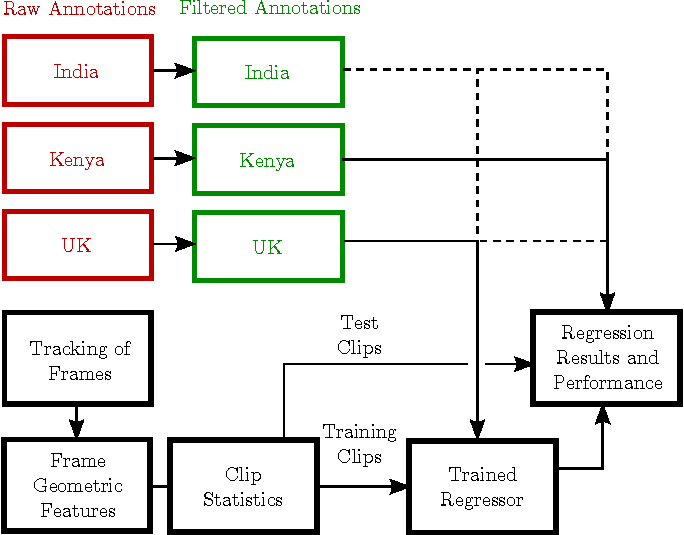
\includegraphics[width = 0.80 \columnwidth]{nvcregression/SystemOverview.pdf}
\caption{Overview of automatic system, showing filtering of annotations followed by training and testing on separate cultures.}
\label{SystemOverviewFigure}
\end{figure}

This section provides an overview of the automatic recognition system. The main steps are depicted in Figure \ref{SystemOverviewFigure}. \ac{LP} tracking is again used (see Section \ref{SectionLpTracking}). The tracking of each frame is then used to create a frame feature $\frameFeature_{alg}$ using the \textit{geometric-a} method (see Section \ref{SectionGenerateAlgorithmic}). The features are normalised on a per-subject basis, as defined in Equations \ref{EqnFeatureComponentMean} to \ref{EqnNormaliseFeatureRange}. For each annotated clip, these frame features are combined into a clip digest vector $\clipFeatureDigest$ using simple statistical measures. Each clip has a single digest vector and a matrix of labels $\filteredAnnotation$ (as described in Chapter \ref{ChapterAnnotation}). Eight fold cross validation is performed by dividing clips into person independent training and test sets. For each training fold, a $\nu$-SVR model is trained for each of the 12 components of $\filteredAnnotation$. The $\nu$-SVR models are then used to predict labels for the unseen samples in the test set. These predicted labels are compared to ground truth and the performance is evaluated by Pearson's correlation (in a similar fashion to \cite{Grimm2007, Kanluan2008}).

The details for feature extraction used to form the clip digest vector will be discussed in the next section, as well as some of the properties of $\nu$-SVR.

\section{\temporalFeatSingleCap{ }Extraction and Regression}
\label{SectionDigestVector}

This section describes the details of the regression system and the differences from the classification approach discussed in Chapter \ref{ChapterClassification}. Tracking and \featureGeneration is used to transform video frames into a form that can be used by standard machine learning techniques. As before, feature point tracking and \featureGeneration are performed by \acl{LP} trackers and \textit{geometric-a} features, previously introduced in Chapter \ref{ChapterClassification}. However these features consider individual frames separately and do not consider how the features vary over time. The clip digest vector, described below, encodes the feature variation over time.

%This section also outlines $\nu$-SVR as a regression technique. Regression is used because, unlike Chapter \ref{ChapterClassification}, the labels are considered as continuous variables.

%Feature generation encodes information about face deformation shape. We do not consider appearance based features, because they did not preform as well as shape features in classification. The LP flock tracking, previously discussed in Section \ref{SectionLpTracking}, is used. This provides position of facial features for the multi-culture annotated video clips (Section \ref{SectionMultiCultitureAnnotation}). We use either heuristic features (Section \ref{SectionGenerateHeuristic}) or algorithmic features (Section \ref{SectionGenerateAlgorithmic}) to create a feature vector which encodes information from a single frame.

\subsection{Computing the Clip Digest Vector by Feature Extraction}
\label{SectionClipFeatureExtraction}

Video clips in the corpus have variable lengths but an automatic system requires a way to compare the similarity of clips. Clip level and frame level performance measurement was introduced in Section \ref{SectionClassificationPerformance}. However, this approach was not particularly satisfactory because the frames were considered in isolation to produce a prediction by decision fusion. It would be preferable to consider how features vary across multiple frames. For this reason, the clip digest $\clipFeatureDigest$ is computed by taking the mean and variance of each feature component. The clip feature matrix $\clipFeature \in \mathbb{R}^{\numClipFrames \times \numFeatures}$, is summarised into a digest vector $\clipFeatureDigest \in \mathbb{R}^{2 \cdot \numFeatures}$. This fixed length vector $\clipFeatureDigest$ may then be used as an input to many standard machine learning tools, including $\nu$-SVR. For feature component $i$, 

\begin{gather}
 \clipFeatureDigest^{\clipId}_i = \overline{\clipFeature^{\clipId}_i}, i \in \{1...\numFeatures\} \\
 \clipFeatureDigest^{\clipId}_{i+\numFeatures} = \varFunc(\clipFeature^{\clipId}_{i+\numFeatures}), i \in \{1...\numFeatures\}
\end{gather}

where $\varFunc(\textbf{x})$ is the statistical variance of vector $\textbf{x}$. This is analogous to temporal quadratic features in Section \ref{SectionTemporalFeatures}, but instead of fitting a quadratic curve to a feature component, a Gaussian distribution is fitted to the frame samples. This decision was also based on the motion of eyes during thinking and the visualisation of feature space in Section \ref{SectionVisualisingGaze}. The main finding of that work was that there is little consistency in eye movement except for overall spread and offset from the origin, which can easily be encoded by taking the mean and variance of features. Neither this digest vector, nor the previous approaches of clip or frame level comparisons consider the order of the frames. However, it would be incorrect to say that these features are not temporal, because they do encode feature variation in multiple consecutive frames. Methods that consider the order of the frames have already been discussed elsewhere (e.g. polynomial features and Akak{\i}n and Sankur's work on \ac{HMM}s and \ac{CRF}s in Section \ref{SectionHmm}). Based on these findings, the claim that the frame order is a panacea for all \ac{NVC} and emotion recognition problems cannot be justified.

\thesiscomment{DISCUSS normalisation of features based on Equation \ref{EqnNormaliseFeatureRange}. This is applied to both feature sets?}

\thesiscomment{DISCUSS the drawbacks that mean and variance are not robust statistics}

\thesiscomment{DISCUSS is this approach only appropriate for clips of limited length?}

\subsection{Support Vector Regression and Performance Evaluation}
\label{SectionRegressionAndPerformanceEvaluation}

$\nu$-SVR \cite{Scholkopf2000} is used to perform regression of \ac{NVC} signals. 
%This technique is related to \ac{SVM}s previously used in Section \ref{SectionSupportVectorMachines}. 
$\nu$-SVR is similar to \ac{SVM}s in that it uses weighted kernels centred on sample points to specify a non-linear transform from feature space to a space that is more suitable. In the case of $\nu$-SVR, the distance from the feature space hyperplane is used to perform the regression, rather than just to separate the space into two regions as done by \ac{SVM}s. As in the case of classification, an \ac{RBF} kernel is used.

\thesiscomment{DISCUSS why RBF and the NU variant?}

%See also classification section \ref{SectionClassificationPerformance}

Because the labels are \continuous variables, the method used to assess performance must be considered. \ac{ROC} analysis, as used in previous chapters, only applies to two class problems. A performance metric that operates on \continuous variables is required. Pearson's correlation coefficient is used, as previously introduced in Section \ref{SectionAnalysisOfMeanRatings}. %This performance metric is sensitive to outliers but insensitive to scale differences between two compared variables. This is advantageous if robustness of the system is critical for an intended application but this measure may be over sensitive if this is not a priority. 
Person independent testing is conducted, rather than multi-person testing, because the person independent case has a broader range of applications than multi-person testing and because it is more challenging. 

\section{Results and Discussion}
\label{SectionRegressionResultsAndDiscussion}

This section discusses the experimental results of the automatic \ac{NVC} regression system. 
%The system was tested using eight fold, person independent cross validation. 
The parameters for $\nu$-SVR of $C = 1.0$ and $\nu = 0.5$ where found to be effective.

\thesisstatement{The NVC be regressed at above chance levels and the performance is comparable to humans(?)}

\begin{figure}
\centering
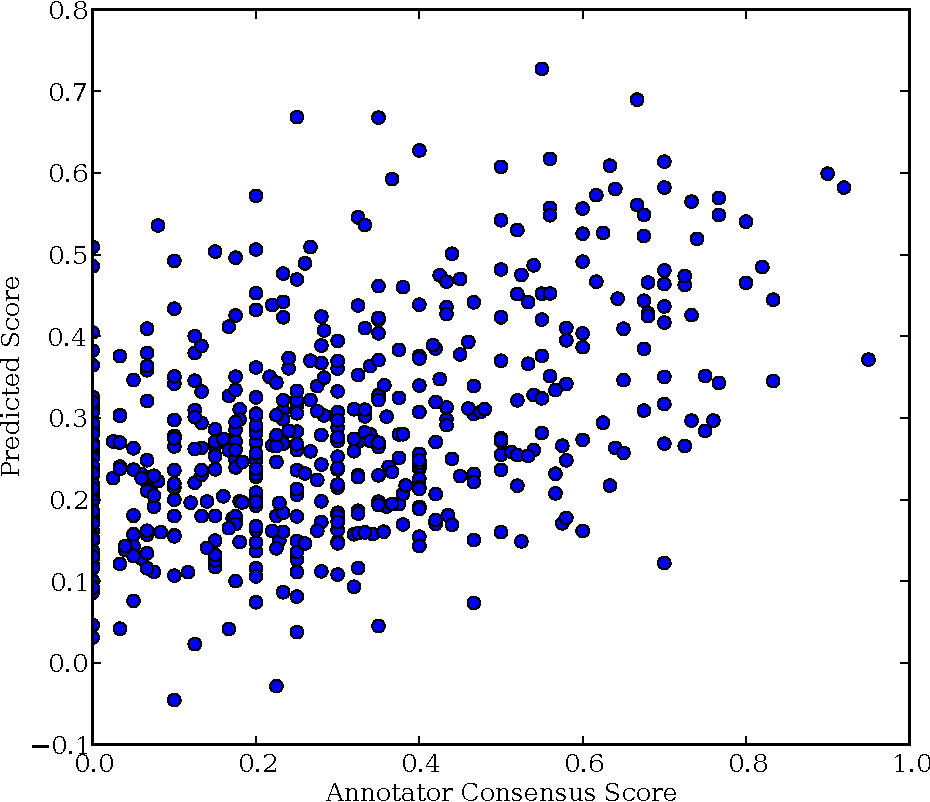
\includegraphics[width = 0.60 \columnwidth]{nvcregression/ScatterThinkUk.pdf}
\caption{Scatter plot of ground truth and automatically predicted \textit{thinking} \ac{NVC} intensities for the \ac{UK} culture. Each point corresponds to a single video clip.}
\label{ThinkScatterFigure}
\end{figure}

The predicted labels and ground truth labels are plotted in Figure \ref{ThinkScatterFigure} for a single \ac{NVC} category (\textit{thinking}) and for a single culture \textit{GBR}. A perfect system would have a linear arrangement of sample points. As can be seen, the distribution of points is certainly not linear, but an overall trend can be observed. 
%The density of points in the bottom left and top right are greater than the top left and bottom right quadrants. 
The Pearson correlation of this distribution is $0.46$ (a score of 1 being perfect correlation and 0 indicating no correlation). There are more samples on the left than on the right area of the plot. This is related to the annotated frequency of different intensity \ac{NVC} signals (see Figure \ref{RatingScoresFigure}). %There is a significant minority of samples that are outliers from the ideal distribution, which is likely to be penalised by Pearson's correlation. However 
The majority of points fall close to where a linear regression line would fall, which implies that most samples have a relatively good \ac{NVC} prediction.

\begin{table}
\centering
\caption[Correlation of automatic system for training and testing on a single culture.]{Correlation of automatic system for training and testing on a single culture. The error limits are one standard deviation of the individual cross validation correlation results. Figure \ref{ThinkScatterFigure} shows the individual ratings for \ac{UK} thinking \ac{NVC}. Note that this table uses a different performance metric than in Chapter \ref{ChapterClassification}, therefore the performance values cannot be directly compared.}
\begin{tabular}{|c| c c c c | c |}
\hline
%Culture & Agree & Thinking & Understand & Question \\
Culture & Agree & Question & Thinking & Understand & Average\\
\hline
\hline
India & 0.38$\pm$0.11 & 0.20$\pm$0.14 & 0.33$\pm$0.13 & 0.23$\pm$0.13 & 0.29\\
Kenya & 0.43$\pm$0.15 & 0.15$\pm$0.19 & 0.39$\pm$0.20 & 0.43$\pm$0.17 & 0.35\\
GBR & 0.27$\pm$0.08 & 0.16$\pm$0.21 & 0.46$\pm$0.20 & 0.37$\pm$0.13 & 0.32\\
\hline
Average & 0.36 & 0.17 & 0.39 & 0.34 & \\
%Global & 0.45$\pm$0.15 & 0.45$\pm$0.19 & 0.50$\pm$0.17 & 0.19$\pm$0.17 \\
\hline
\end{tabular}
\label{CultureCorrelationTable}
\end{table}

\thesisstatement{Different cultures have different NVC regression performances}

Figure \ref{ThinkScatterFigure} shows only one of the \ac{NVC} signals and in a single culture. With annotation data from multiple cultures on four \ac{NVC} categories, the performance of different \ac{NVC} signal regression models can be compared. As can be seen in Table \ref{CultureCorrelationTable}, the performance of some \ac{NVC} signals is low, particularly \textit{question} \ac{NVC}. The difficulty of \textit{question} recognition was previously seen for classification in Section \ref{SectionNvcClassificationResults}. Similarly, \textit{thinking} has the best performance in both regression and classification (see Table \ref{TableAlgorithmicFeatures}). This is unsurprising because both approaches use similar \featureGeneration and machine learning techniques. 
%This may be be caused by \ac{NVC} signals, such as \textit{question}, which rely on a verbal component which is not used in this system. 
Intense expressions of \textit{question} \ac{NVC} are relatively rare in this corpus and the regression algorithm may have difficulty learning a general model if insufficient positive samples are provided. In contrast, \textit{thinking} is relatively common and has a distinct visual appearance, making it easier for a visual system to recognise (see Section \ref{SectionVisualisingGaze}).

Each culture has a different average performance. This may be because one or both of:

\begin{itemize}
 \item the culture's annotators use facial features that are encoded with varying degrees of success by \textit{geometric-a} features.
 \item the quality of annotation varies across culture. IND culture had the largest proportion of untrusted annotators (see Section \ref{SectionAnnotationFilterMethod}) which might indicate a quality problem. It is also possible that different cultures may contain different levels of diversity in \ac{NVC} perception which may affect the validity of the consensus labels $\filteredAnnotation$.
\end{itemize}

%The performance may also be related to the quality of the annotation data.
The annotation labels are based on a mean consensus score $\filteredAnnotation$ for each question (described in Section \ref{SectionAnnotationFilterMethod}). However, individual annotators often differ from these consensus ratings. The human annotator correlation with the culture consensus is shown in Figure \ref{MeanAnnotatorCorrelationTable}. It is questionable if exceeding these performances would be meaningful, because the labels would not correspond to any specific, observable human perception of \ac{NVC}. The human correlation therefore provides an upper ceiling on the performance of our automatic system. This could be addressed by having a focused subset of annotators that have a higher inter-annotator agreement.

The performance of \ac{NVC} signal recognition is at an intermediate level and certainly far from being a reliable prediction. This is due to the extremely challenging nature of the task. The confounding factors include:

\begin{itemize}
 \item most \ac{NVC} signals are quite subtle and can be masked by larger face deformation cause by emotion and head pose changes,
 \item human behaviour in spontaneous conversations is much more variable than posed behaviour (Section \ref{BackgroundWhyIsNvcDifficult}), so the feature space to label partitioning is likely to be complex,
 \item spontaneous behaviour is hard to track, which increases input noise and
 \item some \ac{NVC} signals are based on verbal information which is not considered in this system.
\end{itemize}

\thesiscomment{DISCUSS variance error bars of scores?}

A system with a performance such as this may be useful for some applications where robustness is not a critical requirement. For example, in video retrieval, a list of candidates for clear examples of \ac{NVC} for a human to make a final section could use a noisy regression system to rank the examples. A wider range of applications could be addressed if better performance can be attained. 
%The issue of performance improvement of automatic systems is discussed again in the next chapter. This section returns to examining performance results, and other conclusions can be drawn from the experiments.

\begin{table}
\centering
\caption{Correlation of performance of the automatic system when training and testing on the same or different cultures.}
\begin{tabular}{ | c | c  c  c | }
\hline
Test & \multicolumn{3}{c|}{Train Culture} \\
Culture & India & Kenya & GBR \\
\hline
\hline
India & \cellcolor[gray]{0.9}0.29 & 0.27 & 0.24\\
Kenya & 0.27 & \cellcolor[gray]{0.9}0.35 & 0.33 \\
GBR & 0.25 & 0.33 & \cellcolor[gray]{0.9}0.32 \\
\hline
\end{tabular}
\label{CrossCulturePerformanceTable}
\end{table}

\thesisstatement{Cultural differences are significant in automatic NVC regression (training on the wrong culture results in worse performance)}

Table \ref{CrossCulturePerformanceTable} considers the case of training the automatic system on annotations from a single culture (either GBR, KEN or IND) and testing on annotations from a second culture (again either GBR, KEN or IND). The table diagonal, marked with a grey background, contain the performance of the system in the case where the training culture matches the test culture. For these tests, the results from different \ac{NVC} categories were combined by taking the average performance of the four \ac{NVC} signal performances. The most important point of this table is the diagonal performance values broadly exceed the performance values that are off diagonal. This shows that training a system in one culture's \ac{NVC} annotation and then testing on a different culture results in a performance loss. 
%This has implications for applications of automatic \ac{NVC} recognition. 
Current practice is to consider automatic \ac{NVC} and emotion recognition systems in a single culture and a single social situation. These results suggest this will not be an optimal approach if the culture specific model is intended to be used in a wider range of cultures. Although this result might be expected based on cross cultural research, this is the first quantitative measurement of the effect. This table also suggests a possible solution to the problem: to train specialised systems on appropriate cultural perception data to achieve better performance. The implementation of a cross culture \ac{NVC} recognition system is one of the primary contributions of this thesis.

\begin{figure}
\centering
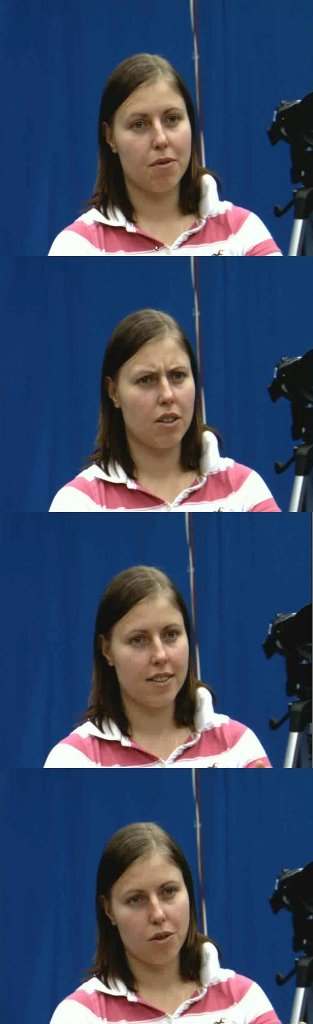
\includegraphics[width = 0.15 \columnwidth]{nvcregression/clip_3dcfiL5Per_col_small.jpg}
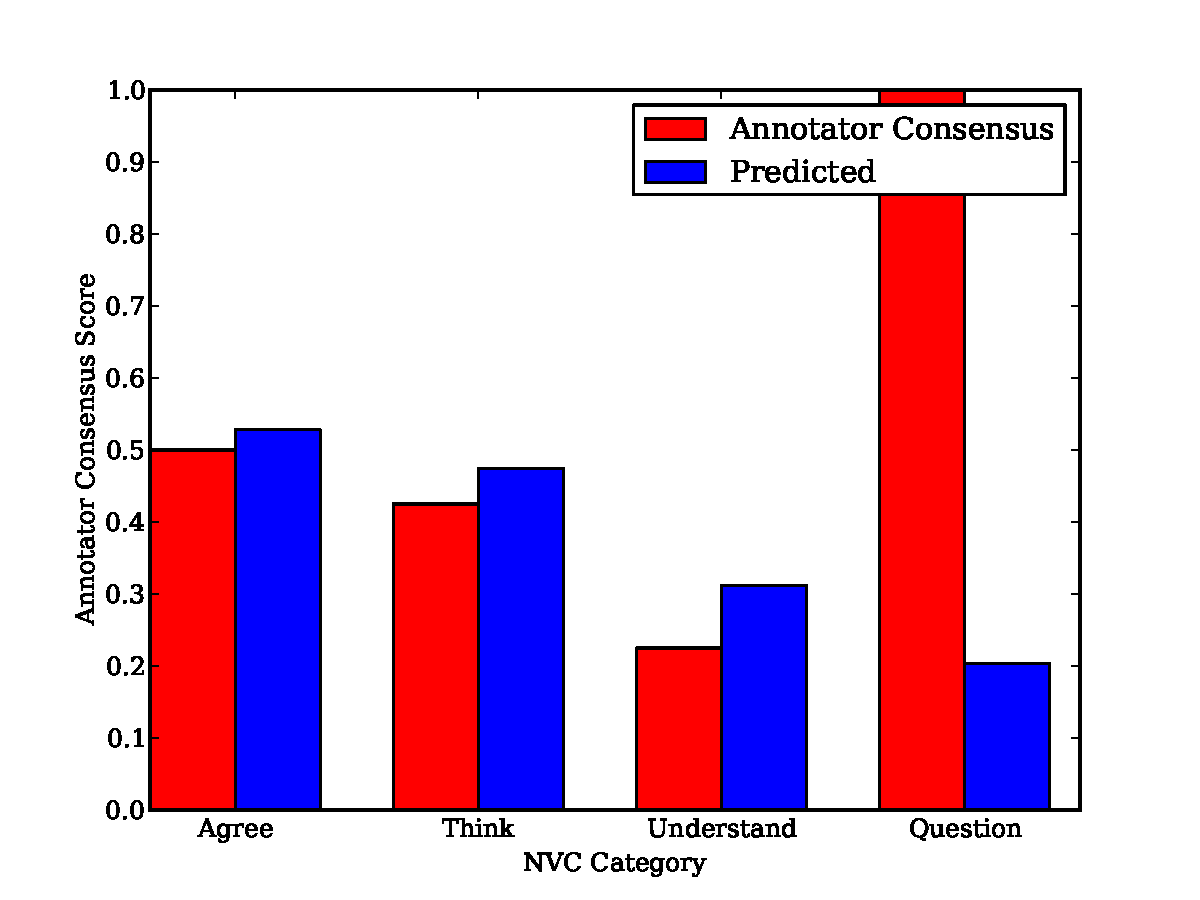
\includegraphics[width = 0.65 \columnwidth]{nvcregression/clip_3dcfiL5Per.pdf}
\caption{Example frames, annotator ratings and predicted scores for corpus clip ``3dcfiL5Per'', in the GBR culture.}
\label{ExampleClipRatings1}
\end{figure}

\begin{figure}
\centering
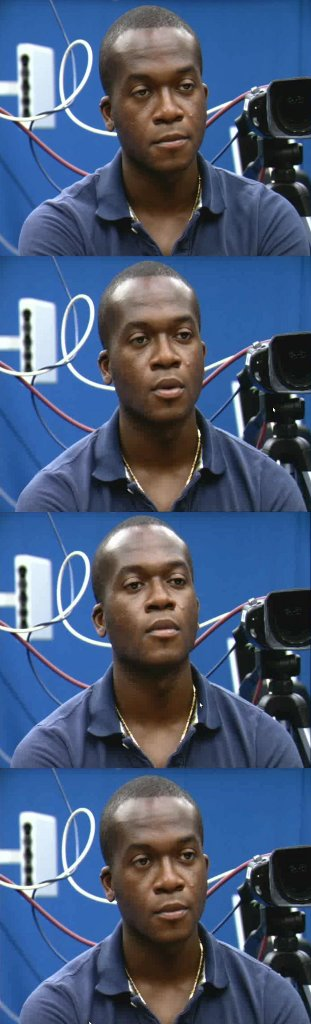
\includegraphics[width = 0.15 \columnwidth]{nvcregression/clip_GyUrjdl6VT_col_small.jpg}
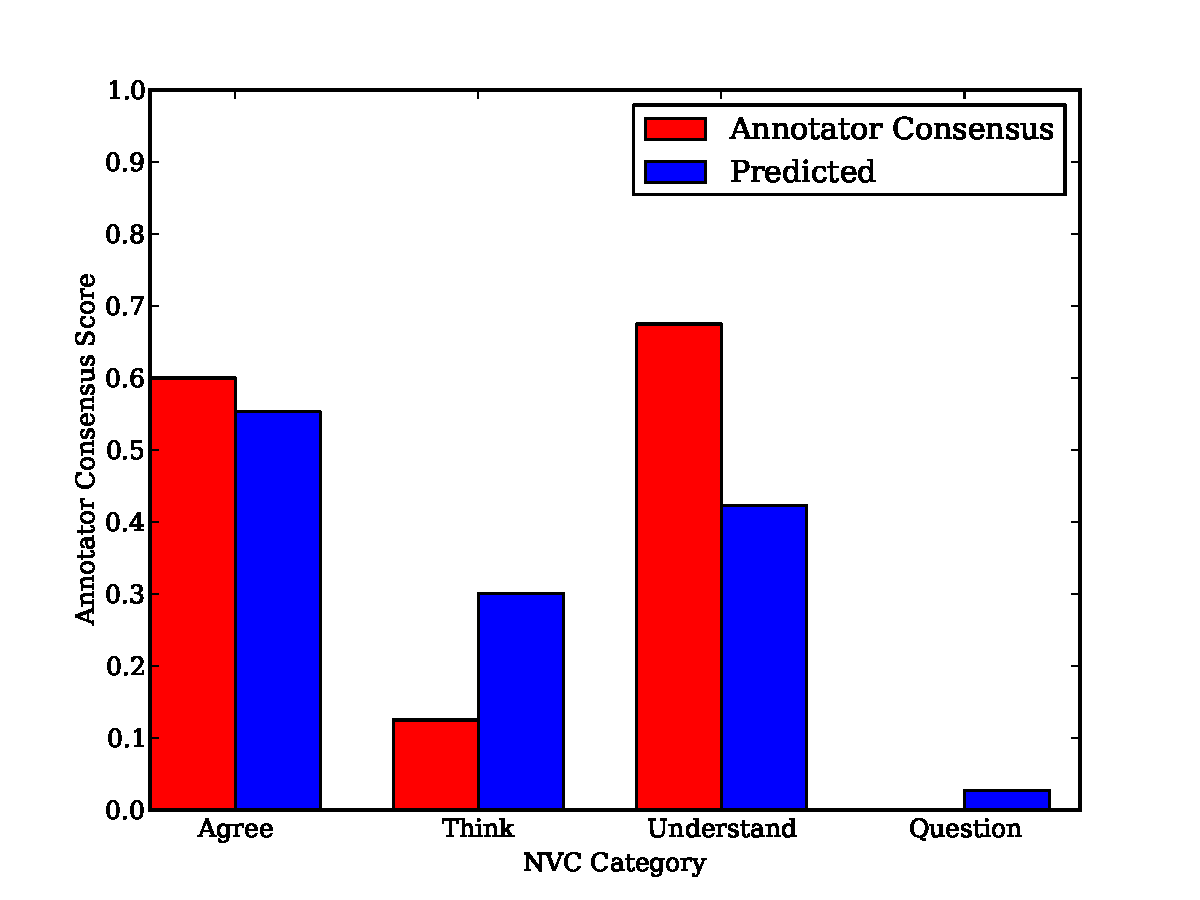
\includegraphics[width = 0.6 \columnwidth]{nvcregression/clip_GyUrjdl6VT.pdf}
\caption{Example frames, annotator ratings and predicted scores for corpus clip ``GyUrjdl6VT'', in the GBR culture}
\label{ExampleClipRatings2}
\end{figure}

To illustrate typical predictions that are made by the automatic system, two random video samples will be examined in more depth. The random video clips are shown in Figures \ref{ExampleClipRatings1} and \ref{ExampleClipRatings2}. The first ``3dcfiL5Per'' clip prediction shows that the predicted (blue) bars are in close agreement with the annotation ratings (red) in three of the \ac{NVC} categories (\textit{agree}, \textit{thinking} and \textit{understand}). However, the annotators have identified this clip as asking a question, resulting in a high score for \textit{question}. The automatic system, has in this case, failed to provide an appropriate prediction.

The second clip ``GyUrjdl6VT'' (Figure \ref{ExampleClipRatings2}) shows that all four predictions are at least approximately correct. The NVC categories \textit{agree} and \textit{question} are almost exactly correct, while the labels for \textit{thinking} and \textit{understand} are in rough agreement. These two figures imply the system is broadly making useful predictions but occasionally has significant errors. 
%This might indicate that some instances of \ac{NVC} are easier to identify than others.

\begin{figure}
\centering
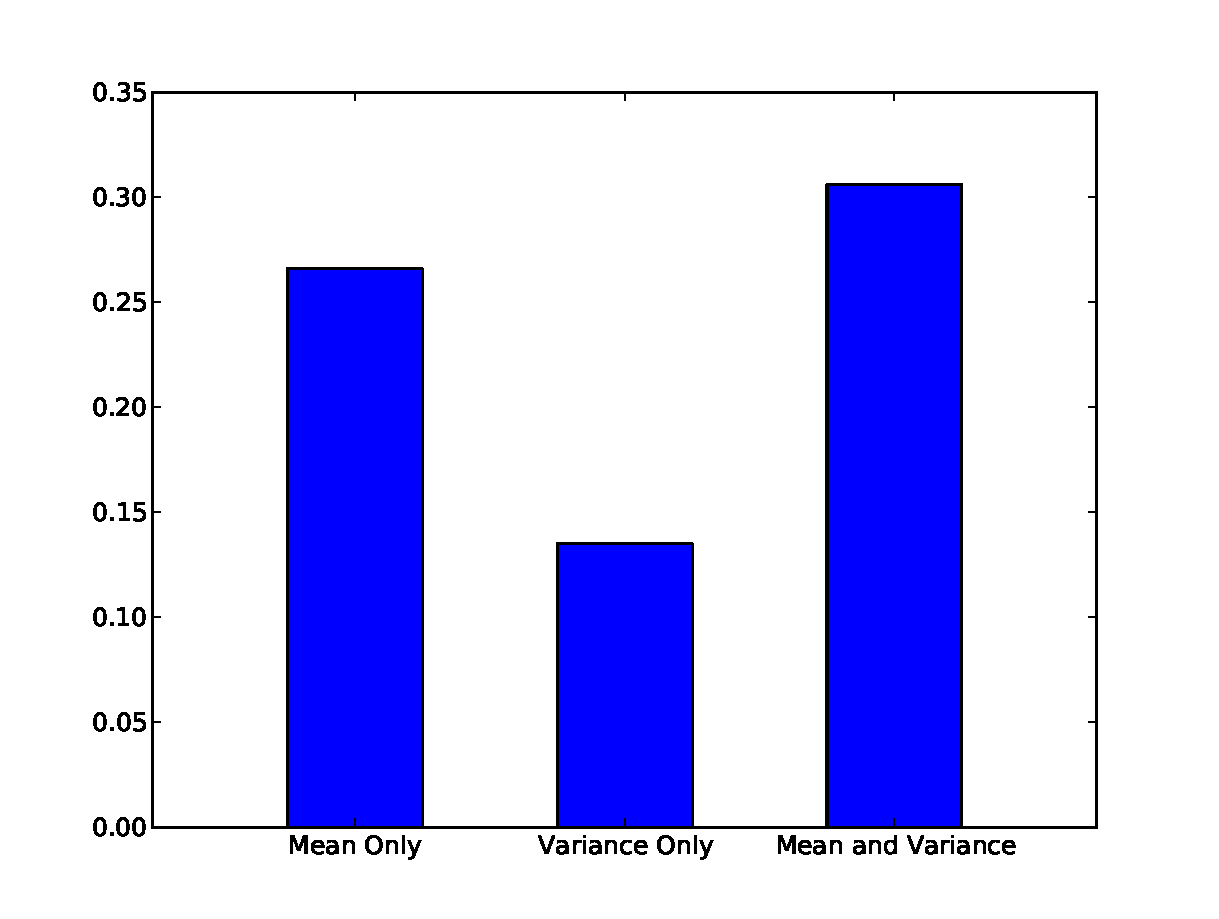
\includegraphics[width = 0.85 \columnwidth]{nvcregression/PlotMeanOrVarianceOnlyFig.pdf}
\caption[The performance of the automatic system using either feature mean statistics or feature variance statistics or the original approach of using both mean and variance statistics.]{The performance of the automatic system using either feature mean statistics or feature variance statistics or the original approach of using both mean and variance statistics. The \ac{NVC} categories and cultures have been combined by taking the average performance.}
\label{FigureMeanOrVarianceCompared}
\end{figure}

As discussed in Section \ref{SectionClipFeatureExtraction}, \featureGeneration was performed by taking the clip mean and clip variance of each component of $\frameFeature_{alg}$. When either the mean features or variance features were disabled, the performance was reduced (see Figure \ref{FigureMeanOrVarianceCompared}). Using only mean based features resulted in a higher performance than just using the variance based features. The mean of features encodes facial expression shape, while variance of features encodes how much motion or activity there is in a local area of the face. This suggests that static face expression contains more information than facial activity for some \ac{NVC} signals. However, there may be more subtle temporal variations that contain relevant \ac{NVC} information. The best performance is when both of these approaches are combined and implies that facial expression and facial activity contain complementary information. Several papers have noted that temporal information is crucial in effective emotion recognition (see Section \ref{BackgroundSupervisedRegression}). Based on the results of this chapter, this holds true of \ac{NVC} as well as for emotion. Perhaps future work can find improved statistical measures that better encode the information to improve system performance.

\begin{figure}
\centering
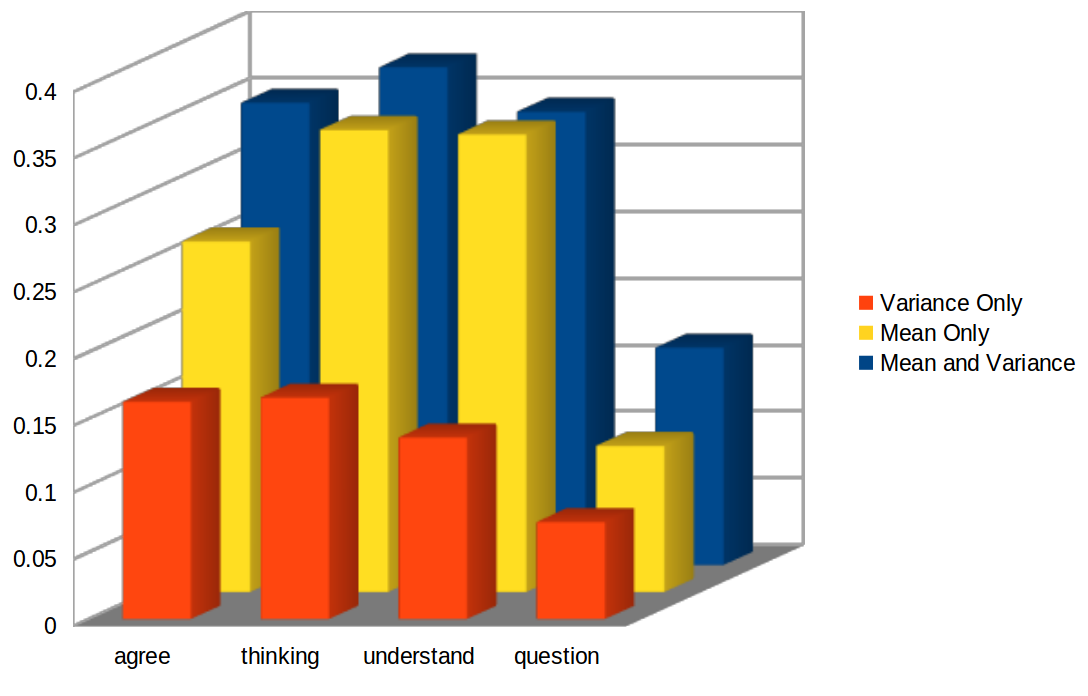
\includegraphics[width = 0.85 \columnwidth]{nvcregression/MeanVarPlotWithCategories.png}
\caption[The performance of the automatic system using either feature mean statistics or feature variance statistics or the original approach of using both mean and variance statistics.]{The performance of the automatic system using either feature mean statistics or feature variance statistics or the original approach of using both mean and variance statistics. Each \ac{NVC} category is separately shown.}
\label{FigureMeanOrVarianceComparedWithCategories}
\end{figure}

The role of facial expression and facial activity can be investigated for individual \ac{NVC} categories. Each \ac{NVC} involves different gestures and different areas of the face. Figure \ref{FigureMeanOrVarianceComparedWithCategories} shows the performance of using only mean statistics or only variance statistics for each category. For most \ac{NVC} categories, both variance and mean statistics provide the best approach for automatic regression. However, the performance for \textit{understand} is approximately equal if the mean statistics approach is compared to the combined mean and variance approach performance. This implies that variance does not contain any complementary information for \textit{understand} \ac{NVC}. It is possible that some \ac{NVC} expressions may be recognized by purely static facial expressions. However, three \ac{NVC} signals require both facial expression and the temporal variation of expression for optimal performance.
%General conclusions are now drawn based on the findings of this chapter.

\section{Applying Digest Vector to \ac{NVC} Classification}
\label{SectionDigestVectorOnClassification}

The concept of encoding a video clip into a fixed length digest vector may also be applied to the person dependent classification problem discussed in Chapter \ref{ChapterClassification}. The approach described in the preceding section is slightly modified to make it suitable for binary class labels and \ac{AUC} performance evaluation. As in Chapter \ref{ChapterClassification}, only clear examples of \ac{NVC} are used, which is a less challenging problem than using all samples in the corpus.

Algorithmic features are generated on video frames and normalised as described in Section \ref{SectionGenerateAlgorithmic}. A digest vector is then computed for each video clip using the method described in Section \ref{SectionClipFeatureExtraction}. A $\nu$-SVC classifier \cite{Scholkopf2000} was trained using two fold cross validation of training and test data. As well as providing a conventional binary label prediction, $\nu$-SVC can provide a prediction of the class membership probability of an unseen sample. This was used in an \ac{ROC} analysis to determine the \ac{AUC} performance.

The performance is sensitive to the $\nu$-SVC cost parameter $C$. The parameter was determined for each fold of the training data independently. Parameter search of cost values of $\{10^{-2},$ $10^{-1},$ $10^{0},$ $10^{1},$ $10^{2}\}$ was performed on the training data on a leave one sample out basis. The cost parameter with the best \ac{AUC} performance was used to train a final classifier on the entire set of train data.

The performance of the system is shown in Table \ref{TableDigestMethodOnClassification}. The changes to \featureGeneration and classification result in a performance increase from 75\% to 85.4\%. This performance is an improvement on the previous state of the art, which was the overall performance of the \ac{HMM} approach proposed by Akak{\i}n and Sankur \cite{Akakin2011}. There are some \ac{NVC} signals, such as \textit{agree} and \textit{understand}, for which \ac{HMM} classification is still more effective than the method proposed here. The overall improvement in performance shows that for some \ac{NVC} signals, appropriate \featureGeneration can effectively encode temporal variations. In some cases, this can exceed the performance of some temporal classifier methods.

\begin{table}[tb]
\centering
\caption{\ac{AUC} performance, expressed as percentages. Testing is on a multi-person basis. The highlighted row corresponds to the method described in this chapter.}
\scriptsize 
\begin{tabular}{ c || c | c | c | c | c }
Method & Agree & Question & Thinking & Understand & Average \\
\hline
Akak{\i}n and Sankur, 2011 \cite{Akakin2011} & 85.9 & 78.2 & 83.8 & 83.6 & 82.9 \\
Sheerman-Chase \etal 2009 \cite{SheermanChase2009} & 70 & 73 & 81 & 80 & 76 \\
Result from Chapter \ref{ChapterClassification} & 70 & 70 & 83 & 75 & 75 \\
\hline
\cellcolor[gray]{0.8}Digest Vector, $\nu$-SVC & \cellcolor[gray]{0.8}81.4 & \cellcolor[gray]{0.8}89.7 & \cellcolor[gray]{0.8}95.8  & \cellcolor[gray]{0.8}74.8 & \cellcolor[gray]{0.8}85.4
\end{tabular}
\normalsize
\label{TableDigestMethodOnClassification}
\end{table}

\section{Regression on High Inter-annotator Agreement \ac{NVC} Signals}
\label{SectionRegressionHighAgreement}

The annotation consensus score $\filteredAnnotation^{\clipId}_{\nvcCategory}$ is formed by taking the mean of trusted annotator ratings. This assumes taking the mean of annotator ratings forms a meaningful \ac{NVC} label. However, the level of inter-annotator agreement, measured by rating variance, is different for each clip (see Section \ref{SectionInterAnnotatorAgreement}). By removal of clips of low inter-annotator agreement, it may be possible to remove data with meaningless labels from the corpus. However, if the filtering is too aggressive, useful and meaningful data may be discarded and the problem begins to become over-simplified.

Experiments were performed based on the method in Section \ref{SectionRegressionResultsAndDiscussion} except that only a subset of clips from the corpus was used for training and test. The subset was based on an inter-annotator threshold. Clips with a higher variance than the inter-annotator threshold were excluded. The system was tested with the inter-annotator threshold at various values. The correlation performance of these experiments are shown in Figures \ref{FigureInterannotatorFilteredPerformanceA} and \ref{FigureInterannotatorFilteredPerformanceB}.

\begin{figure}
\centering
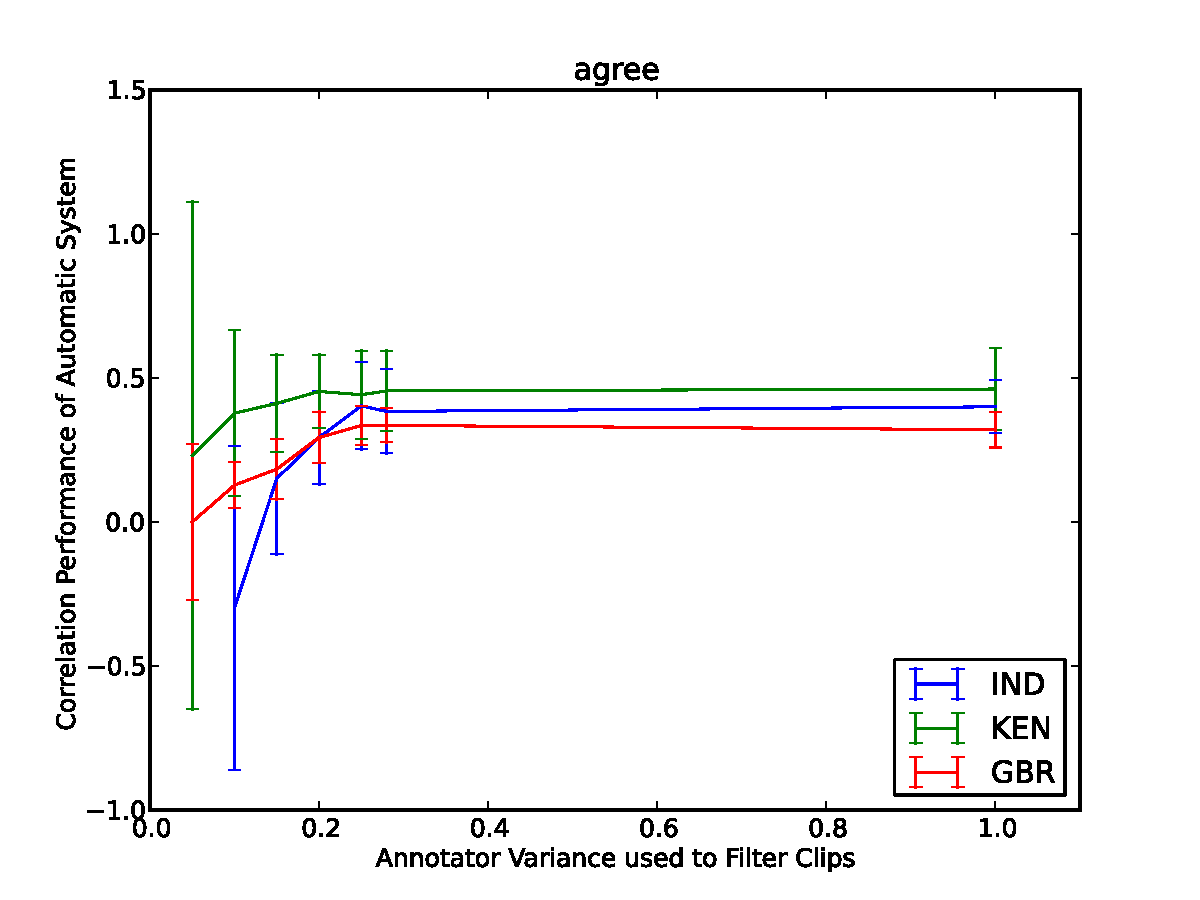
\includegraphics[width = 0.49 \columnwidth]{nvcregression/interannotator/clipfilterperf-agree.pdf}
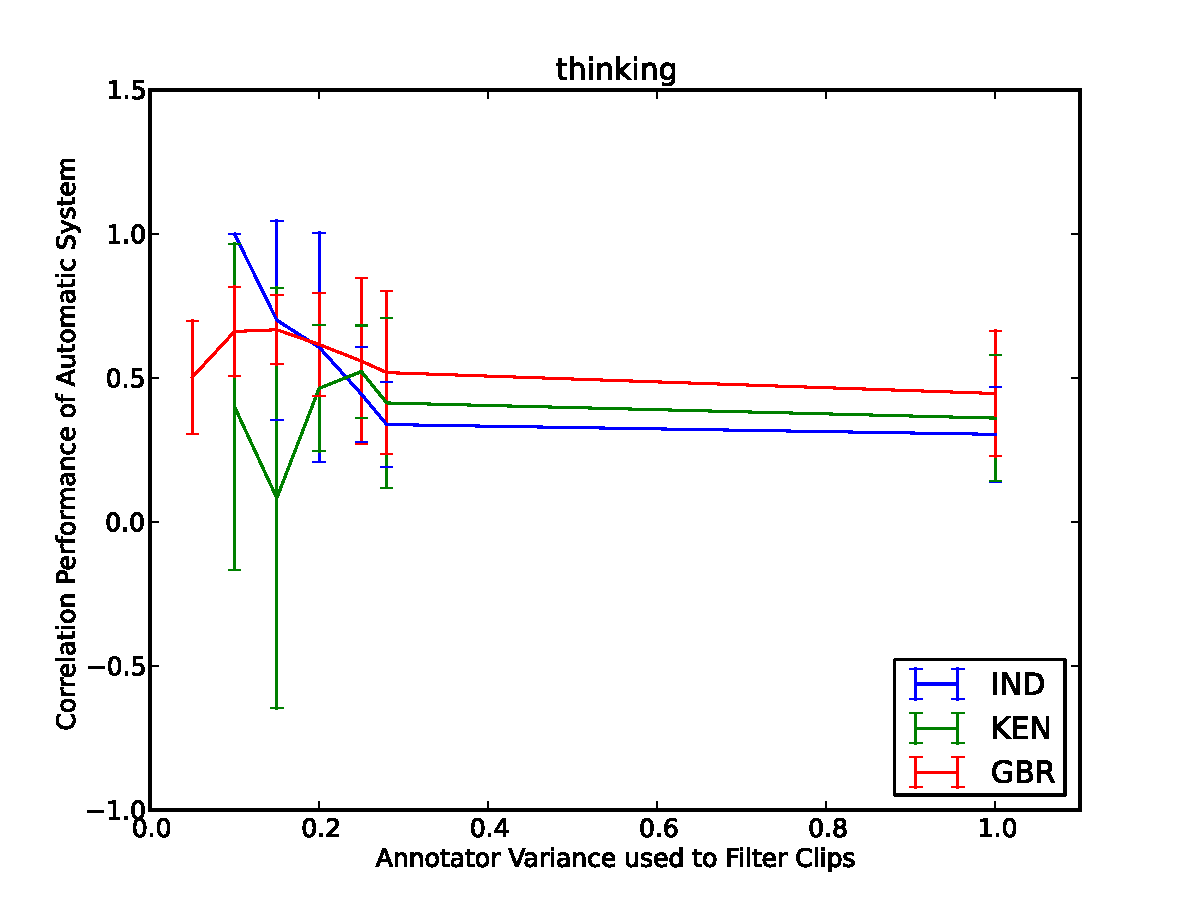
\includegraphics[width = 0.49 \columnwidth]{nvcregression/interannotator/clipfilterperf-thinking.pdf}
\caption[Correlation performance of automatic system after clips with a low inter-annotator agreement have been removed.]{Correlation performance of automatic system after clips with a low inter-annotator agreement have been removed. The left plot shows \textit{agree} and the right plot shows \textit{thinking}. Error bars of one standard deviation are shown.}
\label{FigureInterannotatorFilteredPerformanceA}
\end{figure}

\begin{figure}
\centering
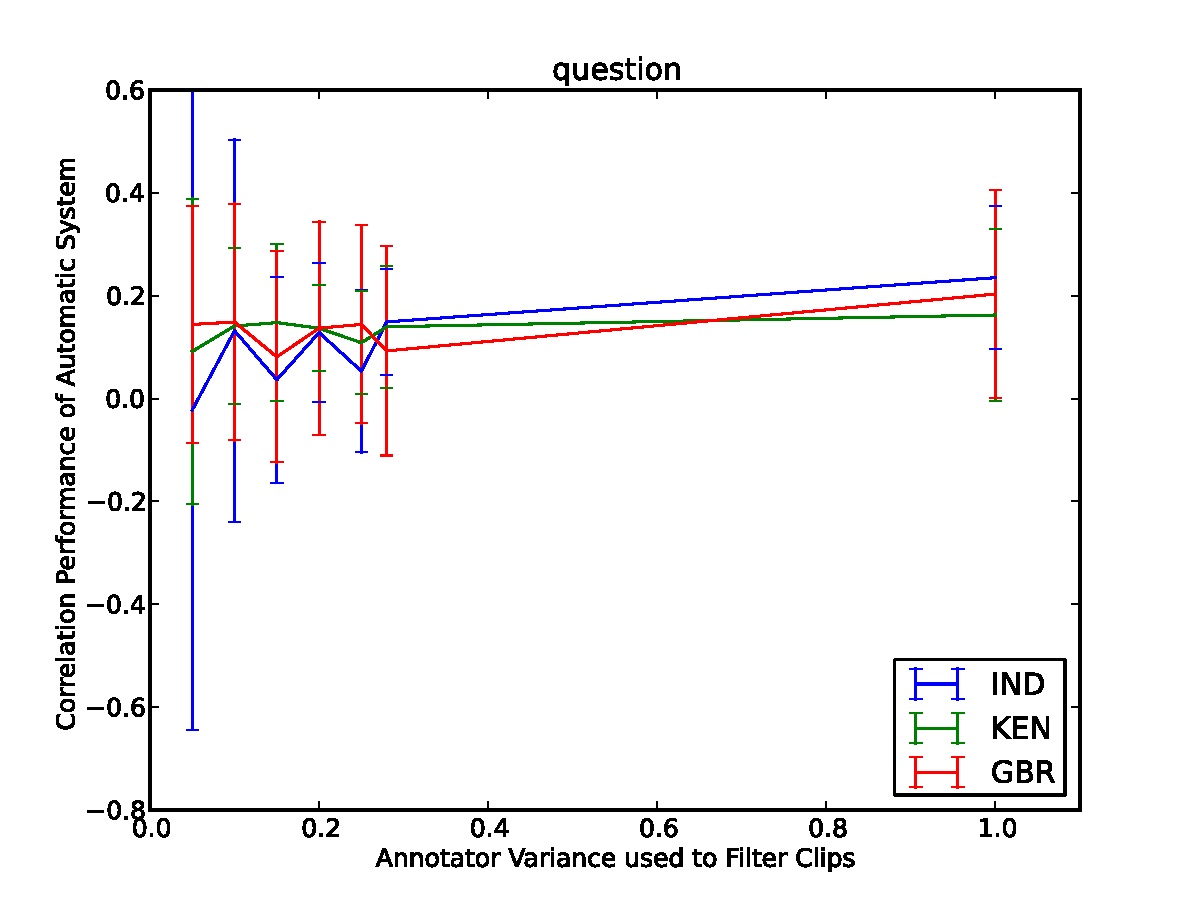
\includegraphics[width = 0.49 \columnwidth]{nvcregression/interannotator/clipfilterperf-question.pdf}
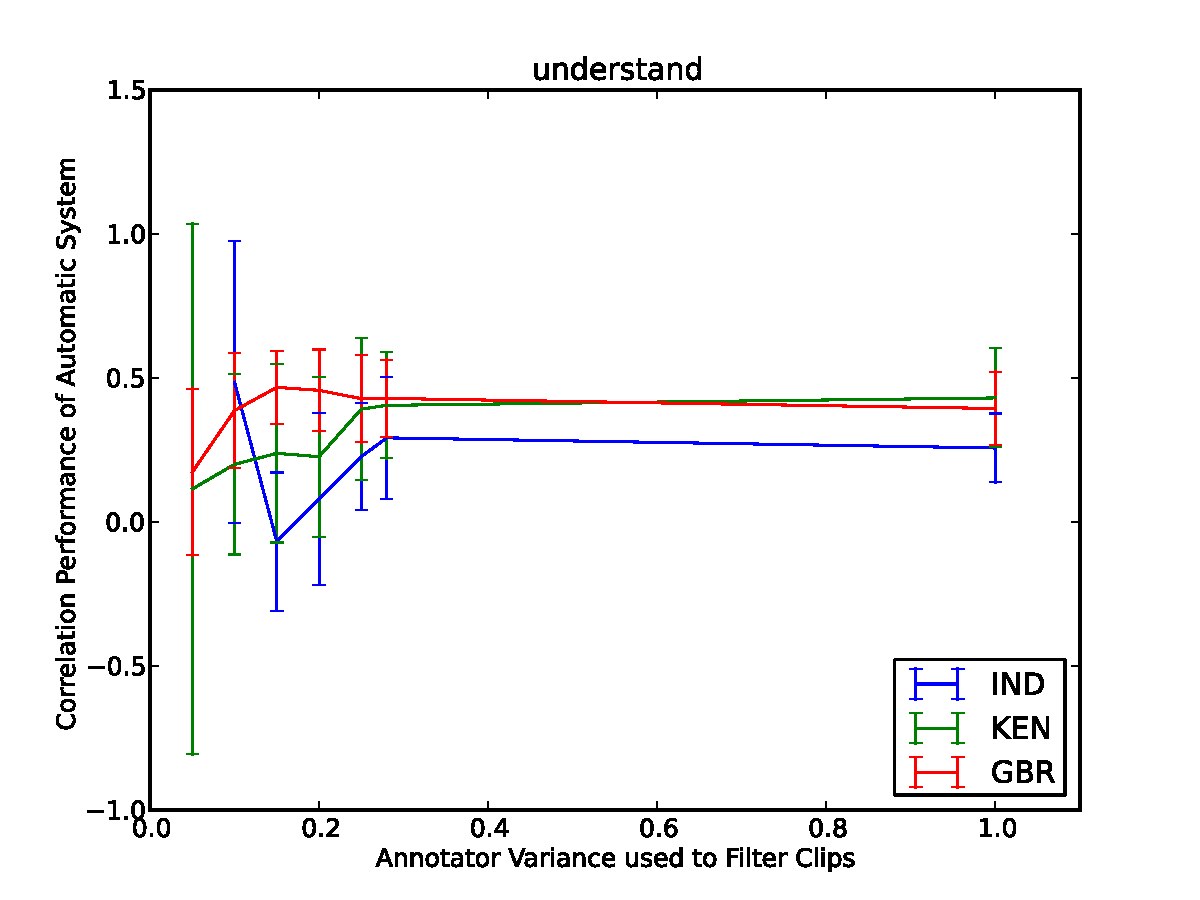
\includegraphics[width = 0.49 \columnwidth]{nvcregression/interannotator/clipfilterperf-understand.pdf}
\caption[Correlation performance of automatic system after clips with a low inter-annotator agreement have been removed.]{Correlation performance of automatic system after clips with a low inter-annotator agreement have been removed. The left plot shows \textit{question} and the right plot shows \textit{understand}. Error bars of one standard deviation are shown.}
\label{FigureInterannotatorFilteredPerformanceB}
\end{figure}

As can be seen in these figures, reducing the threshold to focus on clips with higher inter-annotation agreement results in little overall change in performance. The greatest positive effect on performance is for \textit{thinking}, which may be due to the removal of ambiguous, multi-mode perceptions that may be present for this \ac{NVC} signal (see Section \ref{SectionInterAnnotatorAgreement}). The effect on \textit{agree} is detrimental, which suggests that the machine learning technique is robust to the label noise that is present, while inter-annotator agreement removes data that is useful for training. The other \ac{NVC} categories show no change or possibly a sight negative impact on performance.

Filtering the corpus based on inter-annotator agreement does not appear to be an effective way of improving performance in this case. It may be interesting to investigate the characteristics of \ac{NVC} samples that have higher and lower inter-annotator agreement, as well as the cause of agreement. The appropriateness of agreement metrics as the basis for machine learning could also be explored further \cite{Reidsma2008Thesis}. At present, we can say that the performance is relatively independent to the level of inter-annotator agreement filtering and this \ac{NVC} corpus contains some ambiguous label data which but this is not significantly detrimental to performance.

\section{Classification of Agreement and Disagreement in the Canal 9 Corpus}
\label{SectionCanal9}

The Canal 9 corpus comprises a series of Swiss/French TV studio political debates with a duration of 42 hours. The debates are between 2 to 4 participants and a moderator. The large number of subjects and the use of a single broadcasted view which has been edited from multiple cameras makes tracking more resource intensive. Having more than two participants and the TV cameras may result in increased head pose changes. The corpus has pre-existing annotation data which specifies the shot start/end and the identity of people in the shot. The quality is broadcast TV with interlaced frames. This annotation has been expanded to instances of agreement, disagreement and neutral by Bousmalis \etal \cite{Bousmalis2011} for a subset of shots that have a total duration of approximately 10 minutes and featuring 30 subjects. It is unclear if these annotations were intended to encode mental states or communicated meaning.

\begin{table}[tb]
\centering
\caption[Classification balanced accuracy performance for agreement and disagreement for the Canal 9 corpus.]{Classification balanced accuracy performance for agreement and disagreement for the Canal 9 corpus. The last two rows are the performance of the proposed method. Chance prediction performance is 50\% accuracy.}
\scriptsize 
\begin{tabular}{ c | c || c }
Classifier & Features & Balanced accuracy \\
\hline
SVM & hand/arm/shoulder gestures & 50\% \cite{Bousmalis2011}\\
SVM & prosody & 50\% \cite{Bousmalis2011}\\
SVM & hand/arm/shoulder gestures \& prosody & 52\% \cite{Bousmalis2011}\\
HMM & hand/arm/shoulder gestures & 43\% \cite{Bousmalis2011}\\
HMM & prosody & 51\% \cite{Bousmalis2011}\\
HMM & hand/arm/shoulder gestures \& prosody & 52\% \cite{Bousmalis2011}\\
HCRF & hand/arm/shoulder gestures & 51\% \cite{Bousmalis2011}\\
HCRF & prosody & 56\% \cite{Bousmalis2011}\\
HCRF & hand/arm/shoulder gestures \& prosody & 64\% \cite{Bousmalis2011}\\
\hline
NuSVC & facial \textit{geometric-h} & 50\% \\
NuSVC & facial \textit{geometric-a} & 51\% \\
\end{tabular}
\normalsize
\label{TableCanal9}
\end{table}

The problem is framed as a two class problem and evaluated in a five fold, ``leave one debate out'' cross validation by Bousmalis \etal \cite{Bousmalis2011}. They approached this problem by audio prosody feature extraction and manual hand/arm/shoulder gesture annotation, followed by training a temporal model classifier (\ac{HMM}s or \ac{HCRF}s) to provide automatic predictions. One static classifier was also used (\ac{SVM}). Their approach is similar to this thesis in that they do not use verbal information. Interestingly, they provide performance data for gestures, prosody and both combined. The performance metric used was balanced accuracy.

The method in this chapter is adapted to the Canal 9 data by using NuSVC\cite{Scholkopf2000} classification, which is closely related to the regression method used earlier. Faces were tracked using an extension of \ac{LP} tracking described in Sheerman-Chase \etal \cite{SheermanChase2013} and \textit{geometric-h}/\textit{geometric-a} geometric features are extracted (see Sections \ref{SectionGenerateHeuristic} and \ref{SectionGenerateAlgorithmic}). The features are normalised on a per-subject basis, as defined in Equations \ref{EqnFeatureComponentMean} to \ref{EqnNormaliseFeatureRange}. Multiple frames are combined by taking the feature component mean and variance as described in Section \ref{SectionClipFeatureExtraction}. NuSVR is used to provide a predicted class label.

The performance are shown in Table \ref{TableCanal9}. Just using the visual modality, including the method proposed in this chapter, results in chance level performance. Bousmalis \etal achieve the best results using prosody and arm gestures with \ac{HCRF}. This is likely to be the only result which is significantly above change, although this needs to be confirmed by more experiments. These results are surprising given the above chance classification and regression results using the TwoTalk corpus. There are a number of possible reasons for this result:

\begin{itemize}
 \item Visual features do not provide enough relevant information for humans or automatic methods to predict agreement and disagreement. (Although seeming not the case for TwoTalk)
 \item The facial area does contain relevant information, but the increase head pose changes and lower resolution of the face (typically 150 by 250 pixels in interlaced video) make tracking and extracting this information difficult.
 \item If relevant facial information is extracted, a non-dynamic model may not be suitable for classification. (Although it was suitable for TwoTalk.)
 \item The Canal 9 social context does not rely on facial behaviour for agreement and disagreement compared to the TwoTalk social context.
\end{itemize}

Judging by visual inspection, the tracking of the Canal 9 data seems to be relatively good. Either poor tracker of the different social context seems the most likely explanation for the poor performance. This raises the possibility that different social contexts require different approaches and even possibly different modalities to achieve effective behaviour or \ac{NVC} recognition. This may be an interesting area of future work.

%What about \cite{Bousmalis2012}?

\section{Classification of Mental States in the Mind Reading Corpus}
\label{SectionMindReading}

\begin{table}[tb]
\centering
\caption[Confusion matrix and classification accuracy of Mind Reading emotional states from el Kaliouby and Robinson \cite{ElKaliouby2004}, Figure 7.]{Confusion matrix and classification accuracy of Mind Reading emotional states from el Kaliouby and Robinson \cite{ElKaliouby2004}, Figure 7. Chance prediction performance is 17\%. Rows correspond to the true label, columns to predictions.}
\scriptsize 
\begin{tabular}{ c || c | c | c | c | c | c || c  }
\hline
mental state&agreeing&concentrating&disagreeing&interested&thinking&unsure&accuracy\\
\hline
agreeing	&\textbf{26}	&4	&0	&1	&0	&3	&76.5\%\\
concentrating	&1	&\textbf{16}	&0	&0	&0	&1	&88.9\%\\
disagreeing	&1	&1	&\textbf{17}	&0	&0	&2	&81.0\%\\
interested	&2	&2	&0	&\textbf{23}	&0	&3	&76.7\%\\
thinking	&1	&4	&0	&3	&\textbf{20}	&3	&64.5\%\\
unsure		&2	&3	&1	&0	&1	&\textbf{23}	&76.7\%\\
mean		&	&	&	&	&	&	&\textbf{77.4}\%\\
\end{tabular}
\normalsize
\label{TableMindReadingEK}
\end{table}

\begin{table}[tb]
\centering
\caption[Confusion matrix and classification accuracy of \textit{geometric-a} algorithmic features classified by NuSVC in one-against-all fashion.]{Confusion matrix and classification accuracy of \textit{geometric-a} algorithmic features classified by NuSVC in one-against-all fashion. Chance prediction performance is 17\%. Rows correspond to the true label, columns to predictions.}
\scriptsize 
\begin{tabular}{ c || c | c | c | c | c | c || c  }
\hline
mental state&agreeing&concentrating&disagreeing&interested&thinking&unsure&accuracy\\
\hline
agreeing	&\textbf{18}	&1	&6	&3	&6	&2	&50.0\%\\
concentrating	&2	&\textbf{2}	&1	&5	&3	&5	&11.1\%\\
disagreeing	&9	&0	&\textbf{3}	&1	&8	&3	&12.5\%\\
interested	&2	&2	&0	&\textbf{20}	&3	&3	&66.7\%\\
thinking	&6	&3	&4	&1	&\textbf{10}	&10	&27.8\%\\
unsure		&2	&1	&3	&3	&8	&\textbf{15}	&50.0\%\\
mean		&	&	&	&	&	&	&\textbf{36.3}\%\\
\end{tabular}
\normalsize
\label{TableMindReadingAlg}
\end{table}

\begin{table}[tb]
\centering
\caption[Confusion matrix and classification accuracy of \textit{geometric-h} heuristic features classified by NuSVC in one-against-all fashion.]{Confusion matrix and classification accuracy of \textit{geometric-h} heuristic features classified by NuSVC in one-against-all fashion. Chance prediction performance is 17\%. Rows correspond to the true label, columns to predictions.}
\scriptsize 
\begin{tabular}{ c || c | c | c | c | c | c || c  }
\hline
mental state&agreeing&concentrating&disagreeing&interested&thinking&unsure&accuracy\\
\hline
agreeing	&\textbf{19}	&1	&6	&3	&4	&3	&52.8\%\\
concentrating	&1	&\textbf{1}	&1	&4	&10	&1	&5.6\%\\
disagreeing	&7	&0	&\textbf{4}	&2	&8	&3	&16.7\%\\
interested	&4	&2	&1	&\textbf{19}	&0	&4	&63.3\%\\
thinking	&8	&5	&5	&1	&\textbf{8}	&9	&22.2\%\\
unsure		&2	&0	&2	&4	&12	&\textbf{10}	&32.3\%\\
mean		&	&	&	&	&	&	&\textbf{32.3}\%\\
\end{tabular}
\normalsize
\label{TableMindReadingHeur}
\end{table}

\begin{figure}
\centering
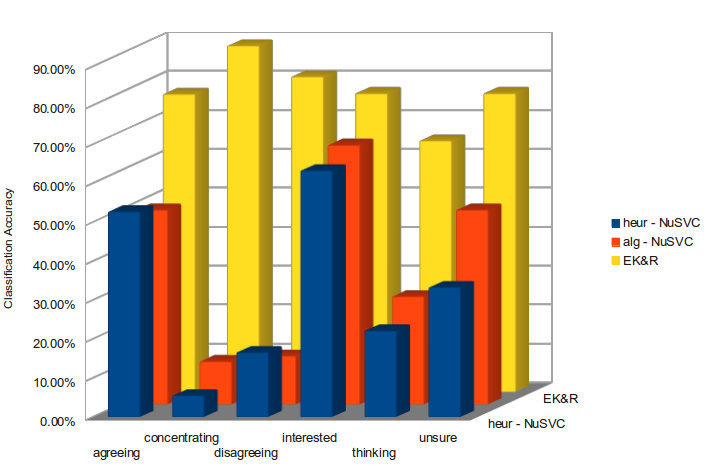
\includegraphics[width = 0.9 \columnwidth]{nvcregression/mindreadingperf.png}
\caption[Classification accuracy for Mind Reading mental states using various methods.]{Classification accuracy for Mind Reading mental states using various methods. Blue bars correspond to \textit{geometric-h} heuristic features classified by NuSVC in one-against-all fashion, orange bars correspond to \textit{geometric-a} algorithmic features classified by NuSVC in one-against-all fashion and yellow bars correspond to el Kaliouby and Robinson \cite{ElKaliouby2004}. Chance prediction performance is 17\%.}
\label{FigureMindReadingPerfSummary}
\end{figure}

Mind Reading Emotions Library is a commercial dataset that was originally developed for assisting those on the autism spectrum. The database comprises of 412 ``concepts'' or classes of mental states. Each concept has 6 silent videos of actors performing the mental state as well as 6 audio recordings. The database was published in 2004 and the video encoding is quite dated, with low quality compression and a small resolution of the face: typically 100 by 150 pixels. el Kaliouby and Robinson \cite{ElKaliouby2004} grouped some of these Mind Reading concepts into an arrangement of 6 classes (see Figure 3.2 in \cite{elKaliouby2005Thesis}). The mental states they studied were \textit{agreeing}, \textit{concentrating}, \textit{disagreeing}, \textit{interested}, \textit{thinking} and \textit{unsure}. This subset has 164 individual clips with a total duration of 19 minutes. These were used to train an automatic system based on a hybrid tracking and appearance features and a multi-scale temporal \ac{DBN} classifier. Ten sequences were discarded because the face tracker did not correctly initialise the head position for the first frame of the video clip. The particular clips excluded was not specified, making a replication of these experiments difficult. Performance evaluation was conducted on a ``leave one clip out'' basis and reported as classification accuracy. Their results are reproduced in Table \ref{TableMindReadingEK}. 

Although the labels in this corpus are superficially similar to the TwoTalk corpus used in this work, the labels of Mind Reading correspond to mental states and not to \ac{NVC} (see section \ref{BackgroundCompareContrastEmotionWithNvc}). However, it is possible to adapt the system proposed earlier in this chapter to the Mind Reading 6 class problem. As before,  features are tracked and \textit{geometric-h}/\textit{geometric-a} geometric features are extracted (see Sections \ref{SectionGenerateHeuristic} and \ref{SectionGenerateAlgorithmic}). The features are normalised on a per-subject basis, as defined in Equations \ref{EqnFeatureComponentMean} to \ref{EqnNormaliseFeatureRange}. Multiple frames are combined by taking the feature component mean and variance as described in Section \ref{SectionClipFeatureExtraction}. NuSVR in a one-vs-all arrangement is used to provide a predicted class label.

The confusion matrices of the proposed method are shown in Tables \ref{TableMindReadingAlg} and Table \ref{TableMindReadingHeur}. A class specific accuracy summary of these results and el Kaliouby and Robinson are shown in Figure \ref{FigureMindReadingPerfSummary}. As can be seen, the performance of the proposed method is significantly lower than that of el Kaliouby and Robinson. In particular, the mental state classes of \textit{concentrating} and \textit{disagreeing} are probably no better than chance predictions. \textit{thinking} is much better than chance, although further experiments are needed to establish the significance of most of these findings. \textit{unsure} and \textit{agreeing} are of intermediate performance but still far below el Kaliouby and Robinson's result. Only the \textit{interested} mental state is nearing el Kaliouby and Robinson's performance. As can be seen in the confusion matrices, \textit{unsure}, \textit{thinking} and \textit{concentrating} are often mistaken for one another. This is hardly surprising, since each of these mental states are very similar in outward behaviour and function. For the proposed method, the \textit{agreeing} accuracy exceeds the \textit{thinking} performance, while for \ac{NVC} the \textit{thinking} was recognized more consistently than \textit{agree} (see Figure \ref{CrossCulturePerformanceTable}). These effects many be cause by:

\begin{itemize}
 \item Acted behaviour is more intense and more consistent than spontaneous behaviour. This may be exploited by the temporal model used by el Kaliouby and Robinson to achieve a better result.
 \item \ac{NVC} and mental states are different concepts. The proposed system was developed for \ac{NVC} and el Kaliouby and Robinson's system was developed to address the Mind Reading corpus.
 \item There is less video data available for each class and more subjects in the Mind Reading corpus, which may affect which method is suitable. Specifically, the proposed method uses subject specific normalisation which can require a significant amount of data to reach a stable and robust model of facial behaviour.
 \item el Kaliouby and Robinson discarded video clips that were not tracked, while we consider all videos, which is a harder problem.
 \item The \featureGeneration technique used by each method is different, which may encode relevant information that is missed by other \featureGeneration approaches. Although the \textit{geometric-h} heuristic features are based on el Kaliouby and Robinson, it is not the same. They use appearance features that focus on mouth opening and teeth visible, which may be useful in distinguishing some of the classes.
\end{itemize}

The performance of the proposed system may be improved by feature selection or by the use of temporal model based classification. This is discussed in Section \ref{SectionMindReadingFeatureSelection}.

\section{Conclusion}

%As discussed in the previous chapter, there are cultural differences in \ac{NVC} perception. 
This chapter describes an automatic system that is trained on \culturallySpecific annotation data. This enables the automatic system to better model the cultural differences in \ac{NVC} perception. The predictions are \continuous labels, which provide richer information than using discrete \ac{NVC} class labels. All clips are used in this chapter, including examples of intermediate intensity \ac{NVC} and are tested in a person independent fashion. Simple geometric features are used, based on distances between pairs of trackers. Temporal information is encoded by taking simple statistical measures of feature components. %This results in an moderately effective \ac{NVC} regression system.

%\ac{NVC} is a subjective domain that is difficult to systematise without unintentionally over simplifying the problem. If a particular \ac{NVC} signal is expressed, it cannot be independently evaluated without human interpretation. 
Human interpretation can only be performed in a specific context. 
%It is difficult to separate cultural differences in expression from the effect of cultural perception with the limited data as used in this study. Also, 
It is difficult to determine if annotation differences are caused by perception differences, or cultural differences in the use of annotation tools. 
%\ac{NVC} signals do not precisely map on to word based concepts. This can make any attempt at translation questionable, if the \ac{NVC} concept being expressed is culturally specific. All these issues makes cross cultural study of \ac{NVC} challenging. 
There are a number of areas in which the current work could be improved. If natural conversations were recorded with \ac{NVC} encoders located in different cultures, effects of perceiving one's own culture vs. perceiving a different culture could be studied. Also, behaviour differences could be investigated, but it may be difficult to ensure each social situation is  equivalent across cultures to enable comparison. Better control of the annotators and encoders would also reduce the possibility that non-cultural effects being the dominant cause in differences of perception. Having the annotators work in a controlled environment and given the same instructions may perhaps improve consistency.

The general approach of specialised modelling of a culture's perception can be scaled to other cultures as long as training data is available. If every possible culture, social situation and personality requires a different model, the high resource requirements to produce these models makes this impractical. However, there are commonalities across social situations and cultures. Therefore, this commonality may be used to adapt an existing model to approximate a new culture or situation without retraining the system from scratch. This process may be similar to adaptation of a speech recognition system to a personalised accent.

Given the evidence that personality and gender affect emotion perception, it is possible these are factors in the perception of \ac{NVC}. Also, annotation data may be gathered without this information being available. It may still be possible to train a tailored system by unsupervised clustering of annotators based on their responses. This would make \ac{NVC} label predictions better reflect actual human responses but the personality type or gender of the annotators would be unknown. %This association between an annotator group and a specialised recognition system may be needed for some applications, but not in others.

The features used are based on an exhaustive extraction of distances between pairs of trackers. This can lead to the inclusion of irrelevant or redundant features, which can cause problems for machine learning algorithms. This can be addressed by feature selection and is discussed in the next chapter.
